\documentclass[color, ddc]{tudscrreprt}
%\usepackage[T1]{fontenc}
% Achtung: LuaLaTeX!!
\usepackage[utf8]{luainputenc}
\usepackage[ngerman]{babel} 
\usepackage{underscore}
\usepackage[colorlinks=false,hidelinks]{hyperref}

\let\myBib\thebibliography
\let\endmyBib\endthebibliography
\renewcommand\thebibliography[1]{\ifx\relax#1\relax\else\myBib{#1}\fi}

\usepackage{floatrow}
\usepackage{graphicx}
\usepackage{caption}
\usepackage{grffile}
\shorthandoff{"}	

\faculty{Fakultät Elektro- und Informationstechnik}
\chair{Institut für Automatisierungstechnik}
\begin{document}
    \title{Dokumentation Praktikum Mensch-Maschine-Systemtechnik}
    \subtitle{Entwurf einer Visualisierung für das
semantische Revisionsverwaltungssystem R43ples}
    \author{Gruppe 2.3:
    Lukas Buntkiel, 
    Alexander Lehmann, 
    Miao Zhang, 
    Sven Schönfeld,
    Falk-Jonatan Strube}
    \maketitle

\tableofcontents

\chapter{Einleitung}

\section{Einordnung}

Hauptbestandteil der Aufgabenstellung ist das Entwerfen einer interaktiven Darstellung der Revisions-Struktur des Versionsverwaltungssystems (Version Control System, VCS) R43ples.

R43ples kann zur Versionsverwaltung von Named Graphs genutzt werden, dem Schlüs\-sel-Be\-stand\-teil des Semantic Web \cite{pascal:semanic-web}. Es verwendet dabei zur Verwaltung der Revisionen wiederum Named Graphs, in denen auch sämtliche, zur Darstellung der Struktur notwendigen, Informationen in Form von Linked Data enthalten sind \cite{graube:r43ples}. R43ples verwendet dabei ein ähnliches Konzept wie klassische Versionsverwaltungssysteme (wie z.B. git \cite{url:git-scm}) indem es Verzweigungen von Revisionen in Form von Branches sowie das Kennzeichnen spezieller Revisionen mit Tags unterstützt \cite{graube:r43ples}.

Der Hauptunterschied zu klassischen VCS liegt also weniger im Konzept der Versionsverwaltung selbst, als in der Anwendung dieses Konzeptes auf einen neuen Typ von Ressource (Named-Graphs). Es kann daher angenommen werden, dass durch andere VCS bereits Lösungen für die graphische Darstellung von Revisionen vorhanden sind, die im Verlauf dieser Arbeit analysiert werden können, um günstige Merkmale herauszuarbeiten.

\section{Theoriebildung}

Die durch den Lehrstuhl gegebene Aufgabenstellung lautet wie folgt:

\begin{quotation}
Ziel dieser Aufgabe ist es, eine gebrauchstaugliche Visualisierung für das semantische Revisionsverwaltungssystem R43ples) zu implementieren, die Revisionsgraphen mit Branches, Merges und Tags darstellen kann. Das Werkzeug soll sich nahtlos in die HTML-Oberfläche des Gesamtsystems einfügen und dem Nutzer Überblicksinformationen über den Revisionsverlauf und Detailinformationen zu den einzelnen Revisionen geben.
\end{quotation}

Dem entsprechend wurden bei der Theoriebildung folgende Kernanforderungen an das Projekt herausgearbeitet.

\paragraph{Schnittstelle zu bestehender Software}

Zuerst muss eine Schnittstelle zur bestehenden Software hergestellt werden. Das wäre möglich, indem man beispielsweise die turtle Datensätze ausliest die der laufende Server ausgibt. Dadurch hätte man ein separates System das unabhängig vom Revisions-Server turtle Datensätze auslesen und darstellen könnte.

Eine andere Möglichkeit stellt die direkte Integration in das R43ples-Projekt auf github dar, in der Visualisierung direkt im System integriert wäre. Diese Herangehensweise hätte den Vorteil, dass man nicht erst eine turtle Datei parsen müsste, sondern direkt auf die Datensysteme des Servers zugreifen könnte. Durch einen fork des repositorys könnte man an einer Lösung der Aufgabe arbeiten und hätte bei einer guten Lösung einen einfachen Weg die Ergebnisse schnell im Hauptprojekt zu nutzen.

\paragraph{Graphische Darstellung realisieren}

Nachdem die Daten für das System über die Schnittstelle beschafft wurden, ist eine Hauptaufgabe diese als graphische Darstellung zu realisieren.

Eine erste Realisierung liegt bereits als einfache Implementierung mit Viz.js vor. 
Diese ist allerdings lediglich als Platzhalter zu bewerten.

Der Graph wird anscheinend nach keinen gestalterischen Grundsätzen generiert. Bis auf die chronologische Auflistung der Revisionen von oben nach unten und die Pfeile als optische Hilfestellung wird keine weitere Hilfestellung geboten, die die Erfassung des Graphen erleichtern würde.

Des weiteren ist die Auswahl der Informationen die von den Revisionen angezeigt werden nicht optimal. Sie bietet dem Nutzer nur zwei Informationen, wobei eine davon für den Nutzer uninteressant ist. Es fehlen aber andere, wichtige Informationen wie beispielsweise der Autor oder das Datum.

\begin{figure}[ht!]
\centering
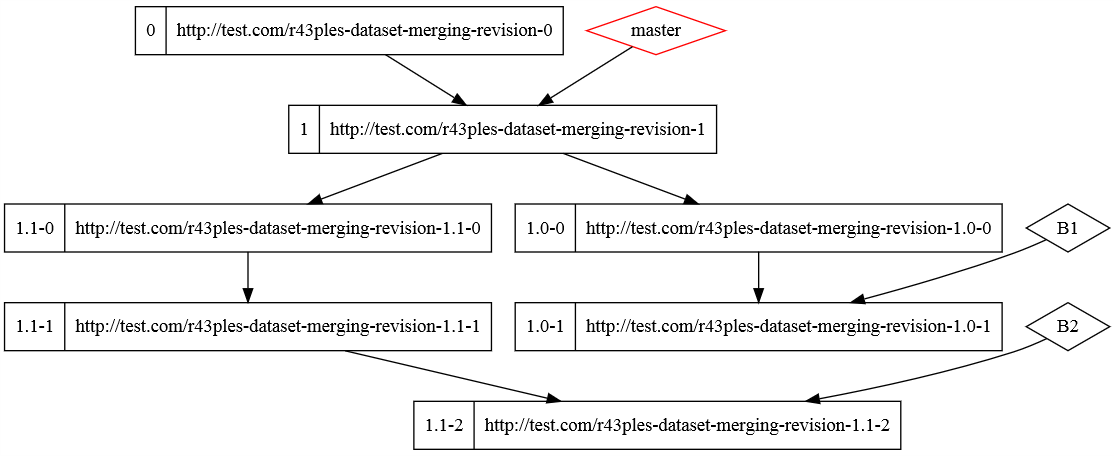
\includegraphics[width=\textwidth]{Skizzen/vizjs.png}
\caption{Vorgegebene Implementierung mit Viz.js}
\end{figure}

\paragraph{Überblicks- und Detailsicht}\label{parag-2ansichten}

Wenn die Idee der vorhandenen Implementierung beibehalten werden soll, die die Informationen der Revisionen direkt in den Knoten des Graphen darstellt, muss überlegt werden, wie bei großen Revisionsbäumen eine übersichtliche Darstellung erreicht werden kann.

Um einen guten Kompromiss aus Informationsfülle und Übersichtlichkeit zu finden würde sich also vor allem bei vielen Daten ein Trennung des Graphen in eine Überblicks- und eine Detailansicht anbieten. So könnte man in einem Überblicksgraphen die wichtigsten Informationen anzeigen und durch das Navigieren auf eine spezielle Revision eine Detailansicht erreichen, die sämtliche relevanten Informationen darstellt.

\subsection*{Wie visualisiert man ein semantisches Versionsverwaltungssystem?}

%Die Frage die sich also stellt ist, wie man ein semantisches Versionsverwaltungssystem am besten darstellt.

Wie bereits in der Einordnung erwähnt, kann als Konzept ein ähnliches verwendet werden wie ein klassischen Versionsverwaltungssystemen. Folgende Richtlinien wurden als Gestaltungsgrundsatz festgelegt:
\begin{itemize}
\item Übersichtlichkeit -- alle wichtigen Informationen sollen mit einem Blick gesehen werden
\item Verständlichkeit -- alle gesehenen Informationen sollen möglichst schnell im Zusammenhang verstanden werden
\item Angemessener Informationsgehalt -- Je nach Ansicht sollen angemessen viele Informationen dargestellt werden nach dem Motto: „so wenig wie möglich, so viel wie nötig“
\end{itemize}

\section{Literatur}

Nachdem in der Einordnung die grundlegende Literatur für das Thema dargelegt wurde (\cite{pascal:semanic-web}, \cite{graube:r43ples}, \cite{url:git}), finden sich auch noch mehr Informationen in verschiedensten wissenschaftlichen Publikationen:

Der Artikel „Special Graph Representations And Visualization Of Semantic Networks“ \cite{borisenko:graph-representation} steigt genau bei der Fragestellung nach der Visualisierung von semantischen Netzwerken ein und bietet einen grundlegenden Überklick für die Herangehensweise.

Die Masterarbeit „Ein empirischer Vergleich von semistrukturierter und unstrukturierter Konfliktbehandlung in Versionsverwaltungssystemen“ \cite{brandl:versionsverwaltung} gibt dabei einen tieferen Einblick zu einem Aspekt der Versionsverwaltung, ist bei der Visualisierung aber nur bedingt hilfreich.

In „Approaches to Visualising Linked Data: A Survey“ \cite{dadzie:linked-data} wird zwar die Visualisierung von Linked Data vorgestellt, allerdings weniger im Bereich der Graphenbildung. Dadurch ist der Artikel für dieses Projekt in dem die Daten durch einen Graphen geordnet darstellen wollen weniger bedeutsam.

Ganz ähnlich bietet „A General Introduction To Graph Visualization Techniques“ \cite{tarawneh:graph-visualization} einen Überblick über die Visualisierungs-Optionen, wobei hier vermehrt Lösungen durch Graphen vorgestellt werden, was den Artikel etwas interessanter für das Projekt macht.

Nach der Theoriebildung bietet sich an nach Literatur zu den gefundenen Problem- und Fragestellungen zu suchen:

Der Artikel „Eye tracking for visualization evaluation: Reading values on linear versus radial graphs“ \cite{goldberg:visualization-evaluation} führt auf, was die Unterschiede sind, ob man Graphen linear oder radial darstellt. Dabei wird der Schluss präsentiert, dass linear dargestellte Graphen deutlich einfacher auf den ersten Blick zu erfassen sind, weswegen in dem Projekt eine solche Darstellung verwendet werden soll.

Die im Internet zu findende Seite „A successful Git branching model“ \cite{driessen:branching-model} zeigt schon auf eine gute Weise, wie man ein Versionsprotokoll darstellen kann und worauf zu achten ist.

Die DIN „Software-Ergonomie für Multimedia-Benutzungsschnittstellen“ DIN EN ISO 14915 \cite{DIN:EN-ISO-14915-1} \cite{DIN:EN-ISO-14915-2} \cite{DIN:EN-ISO-14915-3} gibt entscheidende Richtlinien für die Gestaltung des Projektes im Rahmen einer Benutzerschnittstelle, was vor allem dann von Bedeutung ist, falls die verschiedenen Ansichten in ihren Zoom-Stufen umgesetzt werden soll.
    
\chapter{Analyse und Entwurf}

Nachdem das Thema eingeordnet, eine Entwurfstheorie entwickelt und dazu Literatur herausgesucht wurde, soll auf dieser Grundlage nun eine Analyse geschehen.

\section{Analyse}

\paragraph{Darstellungen anderer Subversion Systeme} Um das Rad nicht neu zu erfinden lohnt es sich die verschiedenen Visualisierungen für die bekannten Versionsverwaltungssysteme GIT und SVN zu betrachten. Dabei werden die Programme GitWeb \cite{url:git}, Gource \cite{url:svn-gource} und Gitready \cite{url:gitready} unter die Lupe genommen. Im Folgenden sollen diese kurz vorgestellt werden.
\begin{figure}[ht!]
\centering
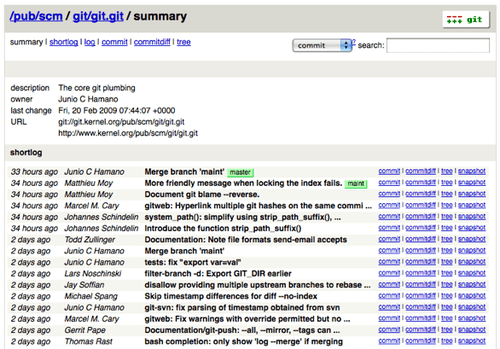
\includegraphics[width=0.4\textwidth]{Skizzen/gitweb.png}
\caption{gitweb Visualisierung}
\label{gitweb-img}
\end{figure}

GitWeb ist eine simple, webbasierte Visualisierung für die Versionsverwaltung GIT. Sie ist im Standardinstallationsumfang von GIT enthalten und stellt die grundlegendste Visualisierungsmöglichkeit für GIT dar. Die Informationen werden dabei tabellarisch in absteigender Reihenfolge ihrer Aktualität dargestellt. In der ersten Spalte wird die Zeit seit dem zugehörigen Commit angegeben. Die zweite Spalte gibt den Namen des Nutzers an, der den jeweiligen Commit durchgeführt hat. In der dritten Spalte wird die Commit-Message wiedergegeben und in der vierten Spalte stehen einige Optionen zur Verfügung (Abb. \ref{gitweb-img}). Die Visualisierung mittels GitWeb ist klar, kompakt und verständlich, allerdings ist die Zugehörigkeit zu einzelnen Branches nicht klar erkennbar, da lediglich Commits zum Master-Branch als solche markiert werden.
\begin{figure}[ht!]
\centering
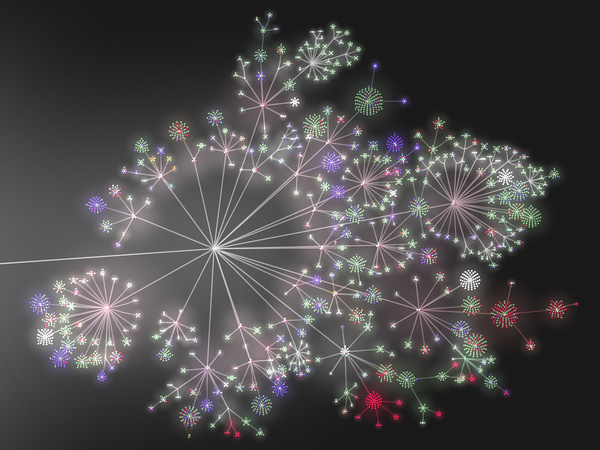
\includegraphics[width=0.4\textwidth]{Skizzen/gource.jpg}
\caption{Visualisierung durch gource}
\label{gource-img}
\end{figure}

	Anders als GitWeb kann das Programm Gource nicht nur mit GIT, sondern auch mit SVN, CVS und anderen verwendet werden. Gource repräsentiert das Dateiverzeichnis als animierte Baumstruktur, bei der das Wurzelverzeichnis im Zentrum liegt (Abb. \ref{gource-img}). Die Blätter des Baumes repräsentieren Dateien. Avatare, die die Entwickler repräsentieren, arbeiten dabei in der selben Reihenfolge wie in der Realität an den einzelnen Dateien und Verzeichnissen, fügen neue hinzu oder entfernen überflüssige. Die Animation kann dabei jederzeit unterbrochen werden. Es werden weder Commit-Messages noch Änderungsdaten angezeigt, der Informationsgehalt der Animation hält sich also in Grenzen. Hierdurch ist Gource eher als Spielerei zur Unterhaltung der Entwickler oder zu Präsentationszwecken zu verstehen, denn als Werkzeug zur Überwachung der einzelnen Versionen.
\begin{figure}[ht!]
\centering
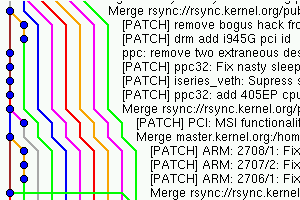
\includegraphics[width=0.4\textwidth]{Skizzen/gitready-gitk.png}
\caption{gitready Visualisierung}
\label{gitready-img}
\end{figure}

	Gitready ähnelt eher GitWeb als Gource. Hier werden die einzelnen Branches als verschiedenfarbige Linien, die parallel nebeneinander auf der linken Seite des Bildschirms verlaufen, dargestellt (Abb. \ref{gitready-img}). Kreise auf den Linien repräsentieren einzelne Commits. Da jeder Commit eine eigene Zeile zugewiesen bekommt ist die Reihenfolge klar ersichtlich. Rechts neben den einzelnen Linien werden die jeweiligen Commit-Messages angezeigt. Auf Grund der Abschnittsweise großen Distanz zwischen Knoten und Message ist das Gesetz der Nähe nicht immer gegeben. Dadurch kann es zu fehlerhaften Zuweisungen zwischen Commit und Message kommen. Allerdings bietet die Darstellung mittels Gitready einen guten Kompriss zwischen Übersichtlichkeit und Informationsgehalt der betrachteten Visualisierungsprogramme. 

\section{Entwurf}	

Bei dem Entwurf stellt sich zunächst die Frage, ob den in der Analyse betrachteten Systemen lediglich nachgeahmt werden soll oder ob neue Ideen einfließen dürfen. Obgleich die Analyse ergeben hat, dass die Visualisierung wie sie von gitready genutzt wird unsere geforderten Qualitäten von „Übersichtlichkeit“, „Verständlichkeit“ und „angemessenem Informationsgehalt“ ausreichend erfüllt, wurde zunächst ein neuer Weg eingeschlagen. Dieser sollte angelehnt an moderne graphische Oberflächen optisch ansprechend sein und dadurch die geforderte Übersichtlich- und Verständlichkeit erfüllen.

\paragraph{Erster Entwurf}
Bei dieser Überlegung ist ein erster Entwurf heraus gekommen, der sich auf folgende Stärken konzentriert (Abb. \ref{entwurf-img}):

Vor allem die Übersichtlichkeit und Verständlichkeit soll durch breit gestaltete Führungslinien zwischen Commits (bzw. Revisionen bei r43ples) sichergestellt werden. Durch die Einordnung in „Spalten“ sollen die Branches eindeutig erkannt werden. Tags sollen zur genauen Zuordnung als wichtige Information direkt am Commit dran stehen.

Als zweite Ebene sollte entsprechend der Idee in der Theoriebildung (Paragraph „Überblicks- und Detailansicht“ in Abschnitt \ref{parag-2ansichten}) eine Detailansicht angezeigt werden. Diese soll sich nach einem Klick auf den entsprechenden Commit öffnet, den Hintergrund abdunkeln und alle wichtigen Details darstellen (Abb. \ref{entwurf_detail-img}).

\paragraph{Probleme beim Entwurf}

Durch den Fokus auf die Benutzerführung durch große Commit-Blätter und breite Zweige ergibt sich allerdings das Problem des benötigten Platzes. Vor allem bei größeren Graphen, wenn nicht mehr der gesamte Graph auf eine Seite passt (oder das Browserfenster verkleinert wurde), würde sich die Übersichtlichkeit ins Gegenteil umkehren.

Zudem wurde aus Gründen des Platzes auch entschieden, dass nicht jedes Commit eine eigene „Zeile“ erhalten kann, wodurch allerdings die chronologische Abfolge nicht gegeben ist und diese Information nicht auf dem ersten Blick zu erfassen ist.

Aufgrund dieser Nachteile wurde sich in der Implementation des Gestaltungsentwurfs dafür entschieden die in der Analyse gelobte Darstellung von GitReady (Abb. \ref{gitready-img}) nachzuahmen. In dieser Darstellung begegnet man den genannten Problemen nicht, hat aber eine vergleichbare Übersicht.


\begin{figure}[ht!]
\centering
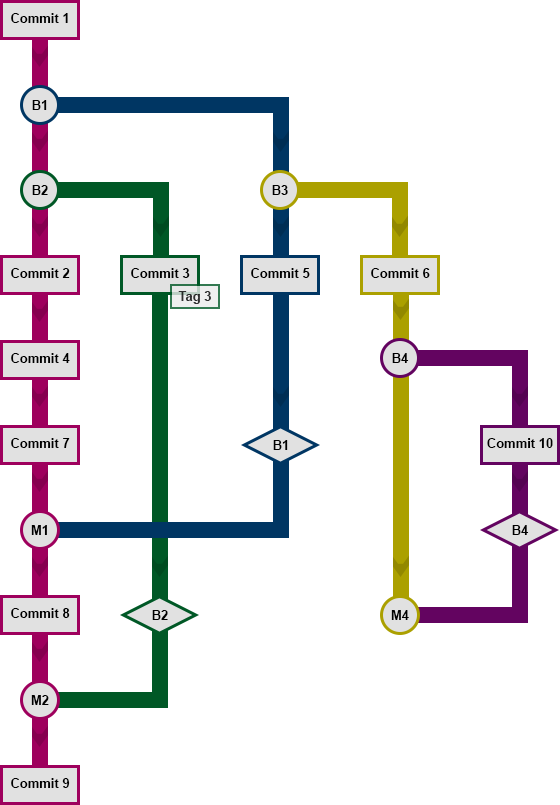
\includegraphics[width=0.8\textwidth]{Skizzen/2015-01 VisualisierungsSkizze-rev.png}
\caption{Skizze für ersten Entwurf}
\label{entwurf-img}
\end{figure}

\begin{figure}[ht!]
\centering
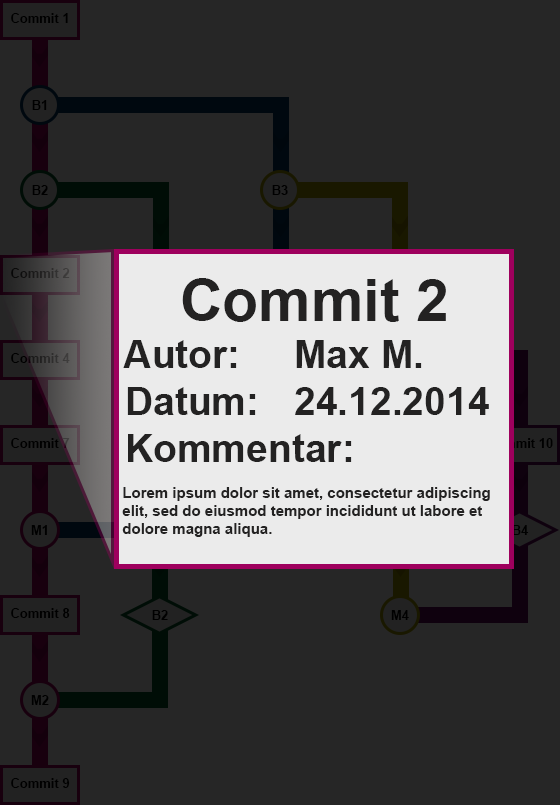
\includegraphics[width=0.8\textwidth]{Skizzen/2015-01 VisualisierungsSkizze-rev_detail.png}
\caption{Skizze für die Detailansicht des ersten Entwurfs}
\label{entwurf_detail-img}
\end{figure}

\chapter{Pflichtenheft}

Im Rahmen des Praktikums erfolgte eine Erstellung eines Pflichtenhefts welches hier nachzulesen ist.

Die Erstellung des Pflichtenhefts erfolgt entsprechend der Empfehlungen des IEEE Guide for Software Requirements Specifications (SRS) \cite{ieee1998ieee}. Die dort empfohlene Struktur wird in deutscher Übersetzung nach Balzert \cite{balzert2009lehrbuch} stichpunktartig knapp übernommen.

\section{Produktfunktionen}
\subsection{Muss}
\begin{itemize}
\item Daten (bspw. aus turtle-Datensatz) auslesen (zum weiterverarbeiten)
\item Daten werden graphisch abgebildet
\end{itemize}

\subsection{Kann}
\begin{itemize}
\item Daten werden in in unterschiedlichen Darstellungsebenen dargestellt (Gesamt- und Detailübersicht)
\item Einzelansicht für die Details von Revisions
\item Daten werden tabellarisch-strukturiert abgebildet
\end{itemize}

\subsection{Soll}
\begin{itemize}
\item Zweckmäßige Übergangsanimationen zwischen Darstellungsansichten
\end{itemize}

\section{Qualitätsanforderungen}
\begin{itemize}
\item Daten werden unverfälscht abgebildet
\item Durch Informationsreduzierung (auf das nötigste) wird ein höhere Übersichtlichkeit erreicht (Minimierung der Darstellung von merges und revisions durch Unterteilung in Detailansichten)
\end{itemize}

\section{Einschränkungen und Randbedingungen}
\begin{itemize}
\item Läuft auf neuerem Firefox und Chrome
\end{itemize}

\section{Annahmen und Abhängigkeiten}
\begin{itemize}
\item Nutzer ist mit r43ples und dem semantic web vertraut
\end{itemize}

\chapter{Gestaltungsentwurf / Implementation}

In der Analyse nach dem ersten Entwurf wurde die Entscheidung für eine Darstellung ähnlich der von GitReady (Abb. \ref{gitready-img}) getroffen.

Der erste Schritt zur Implementation war das github-Projekt zu forken und alle benötigten Dienste (Virtuoso) zu installieren um es in der eigenen Entwicklungsumgebung (eclipse) lauffähig zu machen.

Im Folgenden sollen einige wichtige (Design-) Entscheidungen aufgeführt werden, die bei der Implementation entstanden sind.

\section{Implementation}

\begin{figure}[ht!]
\centering
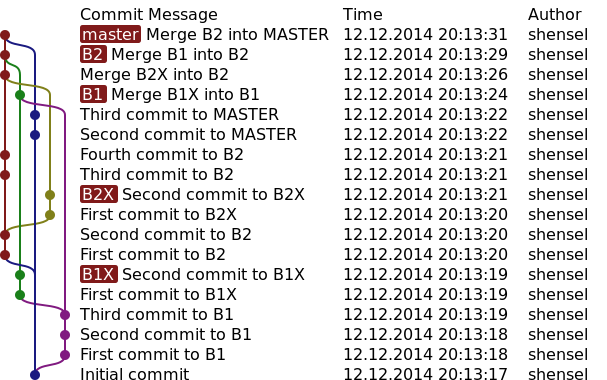
\includegraphics[width=0.6\textwidth]{Skizzen/revisiongraph.png}
\caption{Das erste Ergebnis der Implementation}
\label{implementation-img}
\end{figure}

\paragraph{Framework}
Zuerst wurde entschieden welches Framework verwendet werden soll, um die Visualisierung darzustellen. Die Ausgabe sollte als svg-Datei erfolgen, da dieses eine flexible Einbindung in die Weboberfläche bietet.

Dem entsprechend wurde das Apache Batik Framework genutzt, da dieses die Java Graphics2D API implementiert und somit Code zum Zeichnen (beispielsweise auf einem AWT Canvas) wiederverwendet werden kann.

\paragraph{Commitgraph}
Der Commitgraph soll durch eine neue Datenstruktur des „StructuredTree“s dargestellt werden, um die Arbeit mit Commits zu vereinfachen. Dieser beinhaltet einen doppelt verknüpften Graphen der Commits, eine Liste der Branches und eine Liste der Tags. Beide Listen haben dabei jeweils Referenzen auf die Commits.

Hierdurch wird die Logik zum Generieren der Datenstruktur aus dem SPARQL Result abgekapselt.

\paragraph{Informationsdarstellung}

Entsprechend der Darstellung von GitReady sollen der Commit-Graph und die Informationen zu den Commits nebeneinander dargestellt werden. Dafür ist es wichtig, dass pro Zeile im Commit-Graphen nur ein Commit dargestellt wird, um die entsprechenden Informationen daneben anzeigen zu können.

Mit dieser „ein Commit pro Zeile“-Regel erzeugt man eine bessere Übersichtlichkeit für den Anwender, da die Beschriftungen nicht die Ausmaße des Graphen vergrößern. Somit bleibt der Graph kompakt und kann mit wenigen Blicken erfasst werden.

Des weiteren ist nur eine geradlinige horizontale Augenbewegung nötig um von Commit\-„Punkt“ im Graphen zur Beschriftung zu gelangen. Somit hat man trotz der Informations-Trennung eine hohe Lesegeschwindigkeit (siehe Literatur \cite{goldberg:visualization-evaluation}).

Der Commit-Graph verläuft in Spalten, wobei pro Spalte ein Branch dargestellt wird. Diese eindeutige Zuordnung der Spalten zum Branch ist ebenfalls ein Gewinn für die Übersichtlichkeit, die durch die Einfärbung der Branches (=Spalten) weiter erhöht wird. Bei der Auswahl der Farben für die Branches wurde außerdem darauf geachtet keine aggressiven oder grellen Farben zu verwenden, um einer Ermüdung des Auges vorzubeugen.

\paragraph{Überarbeitung für weniger Redundanz}

Nach einer ersten Implementationsphase wurde das Ergebnis (Abb. \ref{implementation-img}) bewertet. Dabei wurde festgestellt, dass es bei der Informationsdarstellung, vor allem bei der Datumsdarstellung viel Redundanz gibt. Für eine besser Übersicht wurde deshalb entschieden die Zeit-Angabe nur noch Tag-genau darzustellen (da die genau Zeit nicht so wichtig ist und bei direkt aufeinanderfolgenden Commits mehr das „welcher vor welchem“ und weniger das „welcher genau wann vor welchem“ zählt).

Herausgekommen ist das in den folgenden Abbildungen beispielhaft dargestellte Ergebnis:

\begin{figure}[ht!]
\begin{floatrow}
\ffigbox{
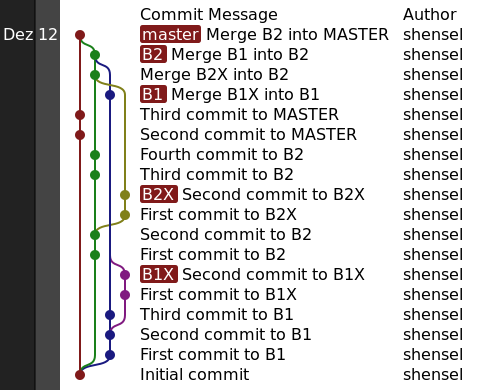
\includegraphics[width=0.4\textwidth]{Skizzen/revisiongraph_http---exampleGraph.com-r43ples-merge.png}}{
\caption{Bsp. Merge-Graph}
\label{imp-f1}}

\ffigbox{
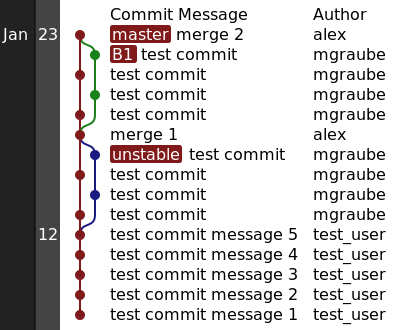
\includegraphics[width=0.4\textwidth]{Skizzen/revisiongraph_http---test.com-r43ples-dataset-1.png}}{
\caption{Bsp. Test Datensatz}
\label{imp-f2}}
\end{floatrow}
\end{figure}

\begin{figure}[ht!]
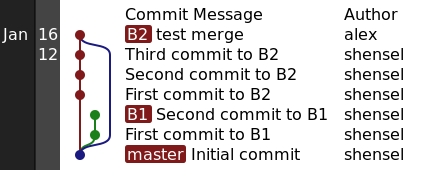
\includegraphics[width=0.4\textwidth]{Skizzen/revisiongraph_http---test.com-r43ples-dataset-merging.png}
\caption{Bsp. zweiter Merge-Graph}
\label{imp-f3}
\end{figure}

Die vollständige Implementation ist im github als fork des Original-Projekts unter \url{https://github.com/flugtiger/r43ples} zu finden.


\section{Ausblick}

Die vorhandene Implementation hat unsere Ziele für das Projekt erreicht: Der Graph für die Darstellung der Revisionen ist  Übersichtlich, Verständlich und bietet einen angemessen Informationsgehalt.

Nach statistischer Erfassung des Nutzerverhaltens und Nutzerbefragungen könnte man noch evaluieren was an der Darstellungsform noch optimiert werden kann. 

Des weiteren könnte die Darstellung beispielsweise durch mouse-over Fenster bei Commits noch mit mehr Informationen gefüttert werden. 

Sollte sich die Lösung für den Kunden als eine gute bzw. die beste der zur Wahl stehenden Lösungen herausstellen, wäre außerdem noch eine nahtlosere Einbindung in die vorhandene graphische Benutzeroberfläche erstrebenswert.
%\chapter{Abgabe}

\section*{Anhang}
Hier sind noch die Programm-Ablauf-Pläne zu finden, die die Funktion der Implementation verdeutlichen:
\begin{figure}[ht!]
\centering
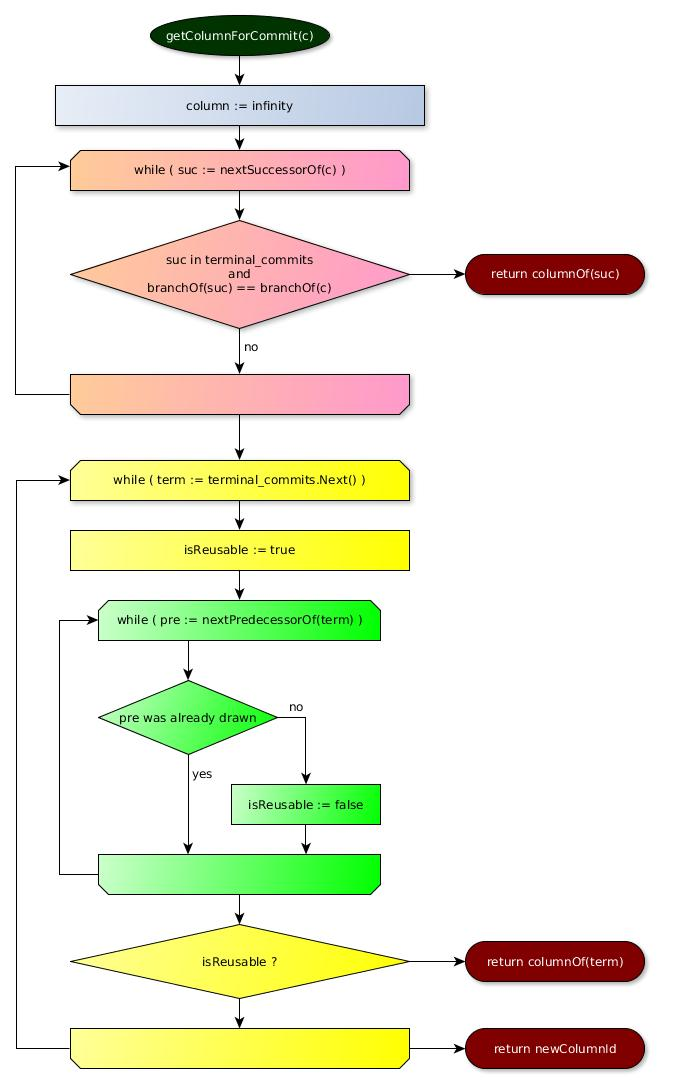
\includegraphics[width=0.65\textwidth]{Skizzen/PAP_getColumnForCommit.jpg}
\caption{Abschnitt des PAPs für die Column-generierung}
\label{pap-column-img}
\end{figure}

\begin{figure}[hb!]
\centering
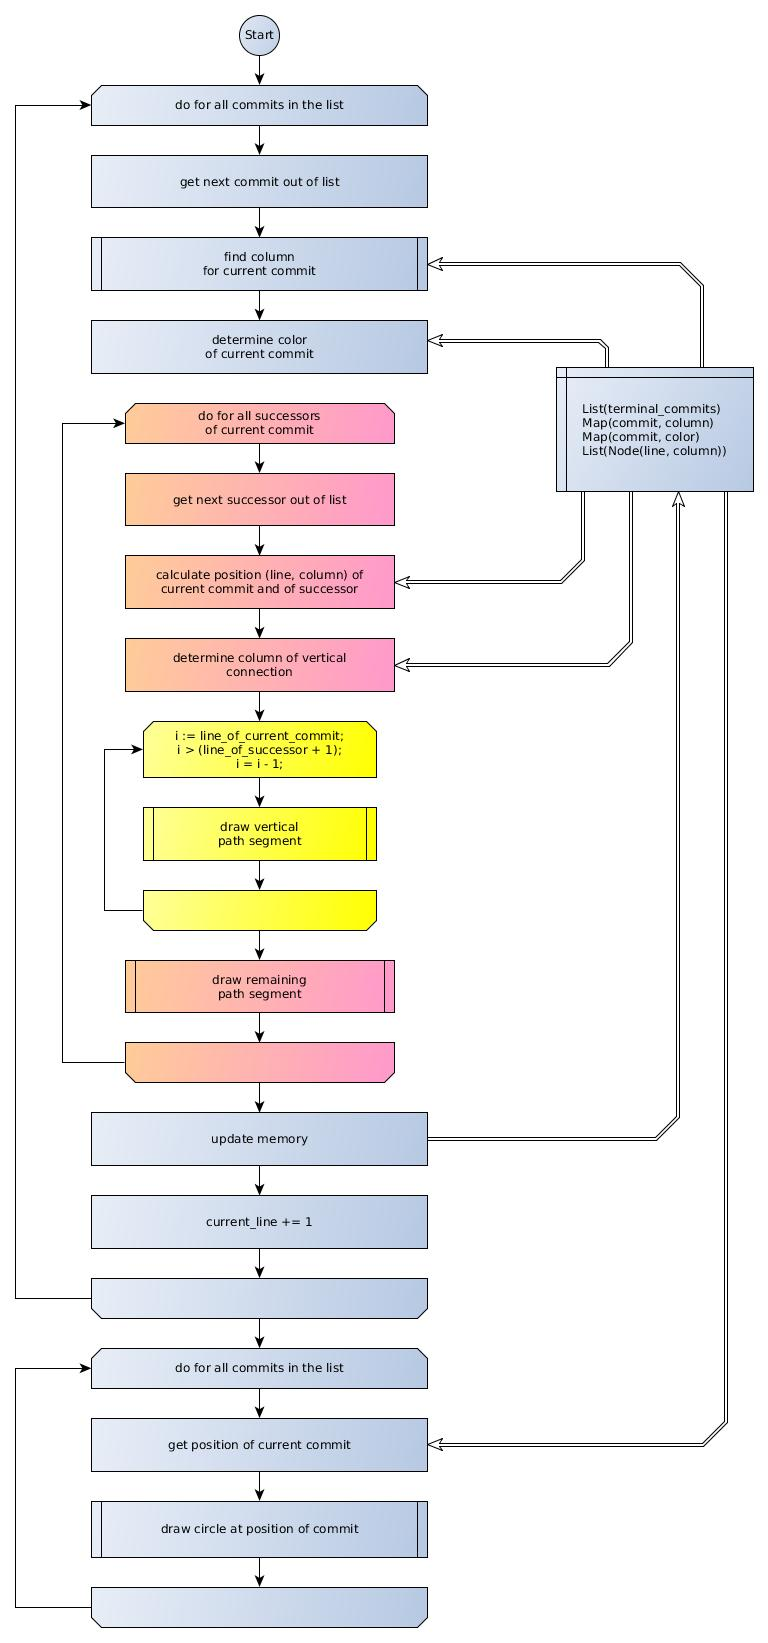
\includegraphics[width=0.65\textwidth]{Skizzen/PAP_gesamt.jpg}
\caption{PAP der Darstellung des Commitgraphs}
\label{pap-img}
\end{figure}


\bibliographystyle{unsrt}
\bibliography{Literatur}

\end{document}